\documentclass{article}
\usepackage{amsmath, fullpage, amsfonts}
\usepackage{graphicx}
\usepackage{siunitx}
\usepackage{float}
\usepackage{bm}


\begin{document}

\title{Progress Report}
\author{Clayton Seitz}
\maketitle
\thispagestyle{empty}


\section{Introduction}

Eukaryotic transcription is episodic, consisting of a series of transcriptional bursts, Bursty transcriptional dynamics are well-exemplified by the transient expression of pro-inflammatory guanylate binding proteins (GBPs) - a group interferon-inducible GTPases that restrict the replication of intracellular pathogens [XXX]. Classical models of gene regulation explain transcriptional bursts by invoking stochastic binding and unbinding of transcription factors, RNA polymerase and mediator proteins at enhancer or promoter sequences. However, more recent studies have pointed towards a more cooperative picture of transcriptional control where phase-separated aggregates of DNA, RNA, and proteins form higher-order structures to control gene expression. For example, both chromatin immunoprecipitation and super resolution imaging have captured the phase separation of super-enhancer-binding proteins MED1 and BRD4 in transcriptional condensates at the \textit{Essrb} genomic locus [XXX]. Furthermore, fluorescence microscopy techniques have colocalized MED1 and BRD4 with the GBP gene cluster alongside a reduction in the degree of disorder of 3D chromatin structure in murine macrophages after infection with \textit{Mycobacterium tuberculosis}. Taken together, these results suggest that phase separation may play a role in the reorganization of chromatin structure during trancriptional control of innate immune response genes [XXX]. Here, we hypothesize that phase separation reduces the entropy of chromatin structure in order to induce bursty gene expression. Using single molecule localization microscopy (SMLM) to obtain super-resolution images of the H2B protein, we intend to demonstrate simultaneous (i) loss of disorder in chromatin structure (ii) formation of transcriptional condensates containing MED1 and BRD4 and (iii) non-Poissonian gene expression. The following sections discuss recent the biological evidence in more detail and summarize the single molecule microscopy techniques and biophysical models we employ to study the interactions between transcriptional condensates and the chromatin scaffold.


\section{Interferon-$\gamma$ induces transcriptional bursts}

\begin{figure}
\centering
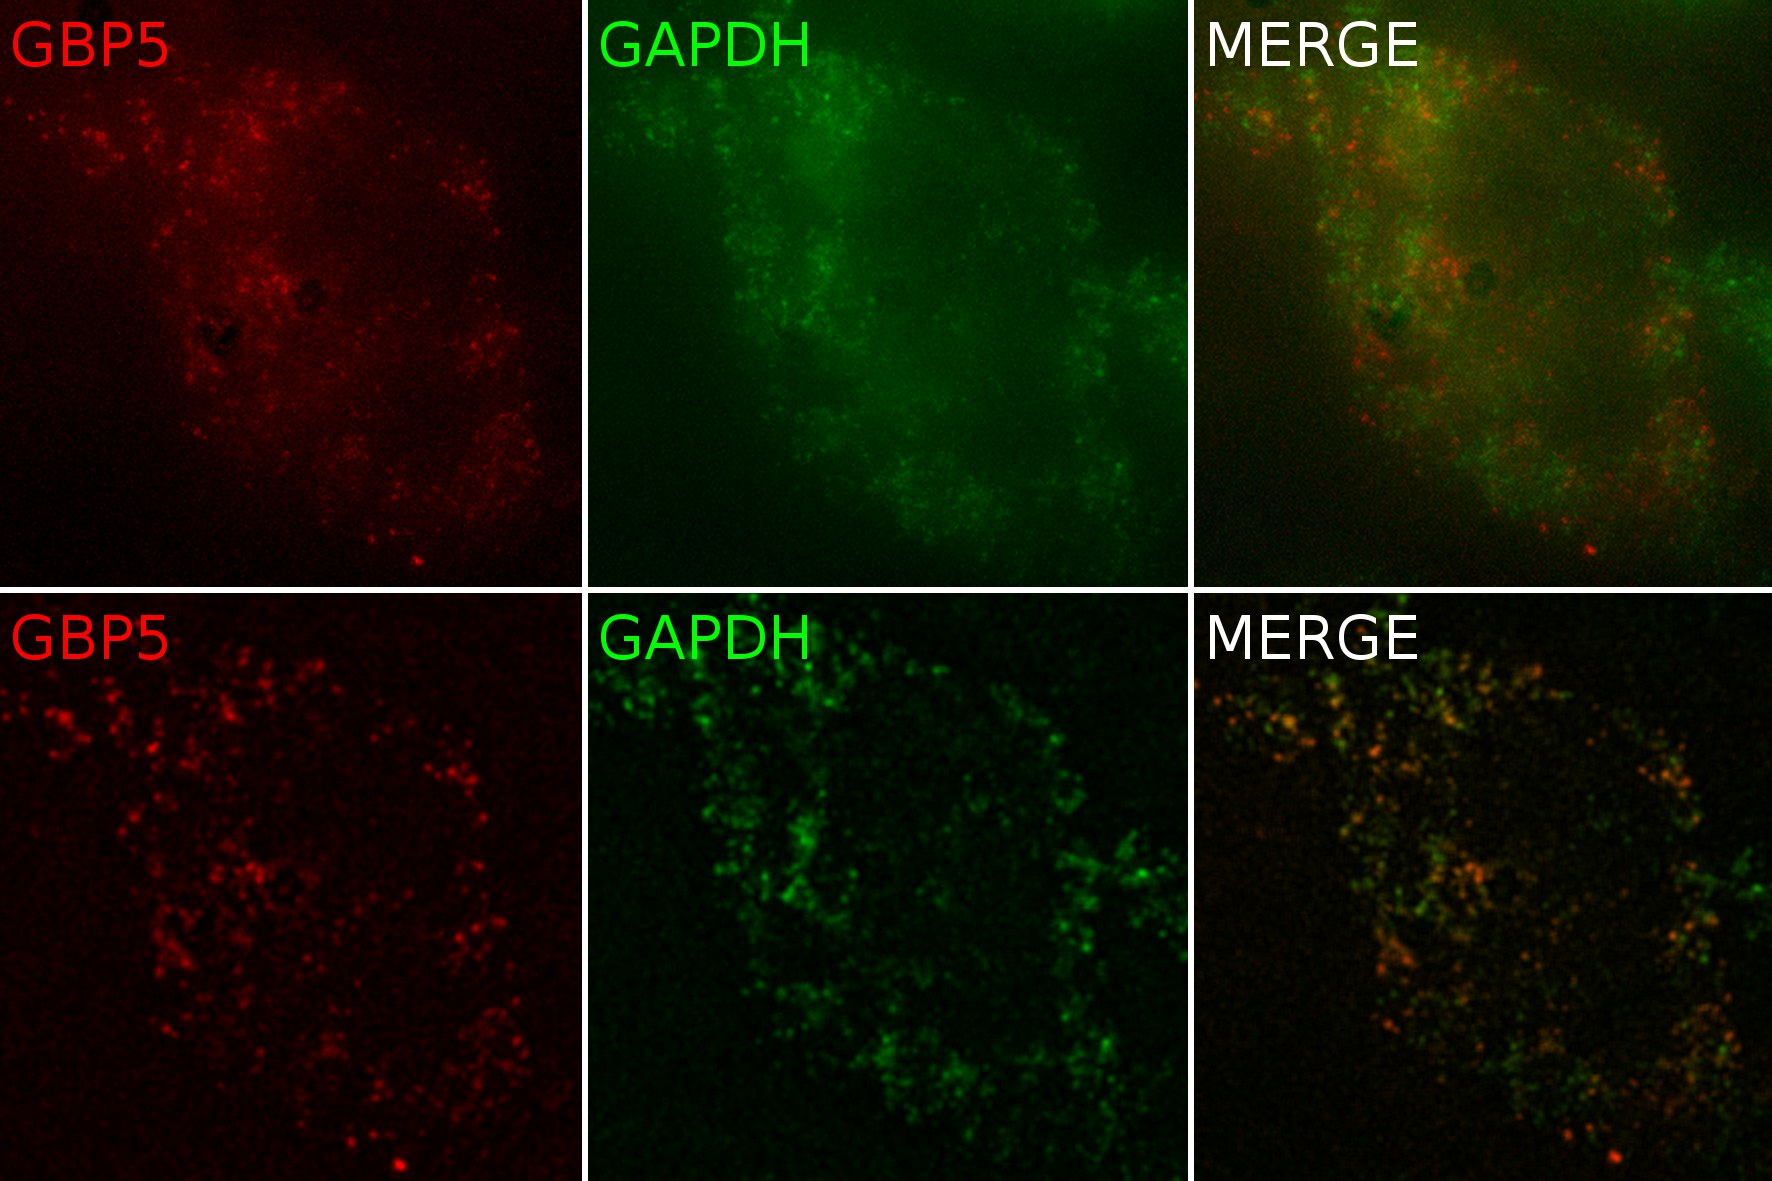
\includegraphics[width=10cm]{Stains.png}
\caption{This will be replaced with histograms}
\end{figure}

Show data analysis for the GBP5 induction experiments
Conclude with perspectives based on recent evidence and bring around what was said in the introduction

\section{Single molecule localization microscopy for superresolution}

According to the Rayleigh criterion, there exists an upper bound on the resolution of the optical microscope due to diffraction. A single fluorescent molecule can, at best, be detected by the fluorescence microscope as a spot 100-200nm in size referred to as the point spread function or impulse response of the lens system. At its core, the Rayleigh limit exists due to overlapping point spread functions, thus creating ambiguity in the localization of individual fluorophores. Single moleculate localization microscopy (SMLM) is a super-resolution method that overcomes the Rayleigh limit by taking advantage of the photoswitching properties of certaint fluorescenct probes under certain chemical conditions. Stochastic photoswitching permits a resolution around 20nm, which is bounded only by pixelation and error bounds of subpixel localization routines, such as point spread function fitting. In general, SMLM has had broad applications in single-cell biology, from super-resolution imaging of the fine structure of DNA, to imaging the structural properties of the cytoskeleton.

Direct stochastic optical reconstruction microscopy (dSTORM) is a SMLM technique that uses conventional fluorescent probes such as labeled antibodies or chemical tags for subdiffraction resolution fluorescence imaging with a lateral resolution of 20 nm. dSTORM experiments start with bright fluorescent samples in which the fluorophores have to be transferred to a stable and reversible OFF state. The OFF state has a lifetime in the range of 100 milliseconds to several seconds after irradiation with light intensities low enough to ensure minimal photodestruction. Then, either spontaneously or photoinduced on irradiation with a second laser wavelength e.g., 405nm, a sparse subset of fluorophores is reactivated and their positions are precisely determined. Repetitive activation, localization and deactivation allow a temporal separation of spatially unresolved structures in a reconstructed image. 

Detectors often suffer from dark noise which follows a normal distribution (central limit theorem). Unless otherwise specified we will always assume that $W_{k} \sim \mathcal{N}(m_{k},\sigma_{w,k}^{2})$. We represent our corrupted signal as another random variable $H_{k}$. As a side note, we define $S_{k}$ to have units of photons $[\mathrm{p}]$, while $H_{k}$ has units of photoelectrons $[e^{-}]$. The conversion factor between the two is the gain of the detector element $g_{k}\; [e^{-}\mathrm{p}^{-1}]$. 
 
\begin{equation}
P(H_{k}) = \frac{\exp\left({-\lambda_{k}}\right)}{\sqrt{2\pi}\sigma}\sum_{n=0}^{\infty}\frac{\lambda_{k}^{n}}{n!}\exp\left(-\frac{(H_{k}-g_{k}n-m_{k})^{2}}{2\sigma_{k}^{2}}\right)
\end{equation} 
 
\begin{align*}
I(\theta_{i}) &= \underset{\theta}{\mathbb{E}}\left[\sum_{k}\frac{\partial^{2}}{\partial\theta_{i}^{2}}  \ell (H_{k}|\theta)\right]\\
\end{align*}

\begin{figure}
\centering
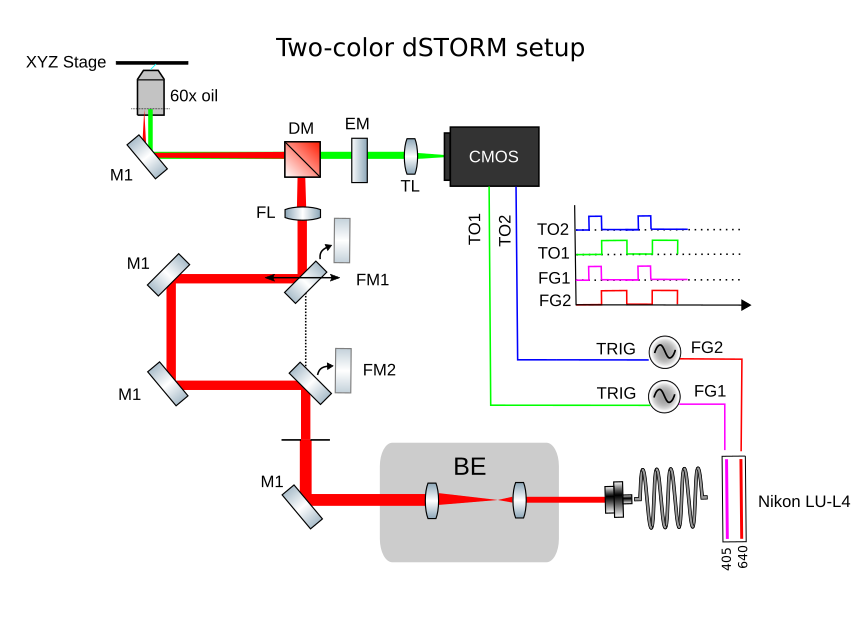
\includegraphics[width=12cm]{dSTORM.png}
\caption{Direct stochastic optical reconstruction microscope}
\end{figure}

\section{Langevin dynamics of a Rouse-like polymer embedded in a transcriptional condensate}

The formation of these transcriptional condensates driven by MED1 and BRD4 alongside decreased entropy of the chromatin scaffold have been previously demonstrated with super-resolution microscopy. Yet, a general biophysical description of the interaction between transcriptional condensates with the chromatin fiber has not been shown and the mechanisms by which they evoke bursty gene expression remains mere speculation. We intend to address these outstanding questions by modeling transcriptional condensate formation within a Rouse-like polymer model parameterized by constraints measured in single particle tracking experiments. These models serve to address the stability of transcriptional condensates as a function of their stoichiometry and the relationship between condensate formation and transcriptional bursting by integrating their associated Langevin dynamics with Monte Carlo simulations. 

\clearpage
\begin{figure}
\centering
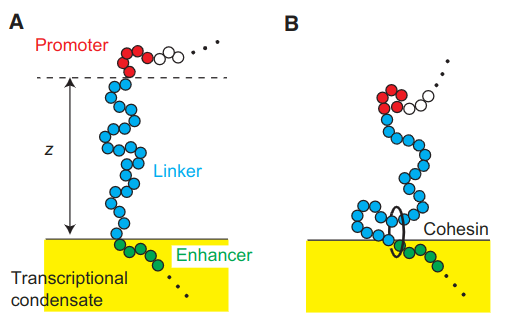
\includegraphics[width=10cm]{Model.png}
\caption{Direct stochastic optical reconstruction microscope}
\end{figure}


\bibliographystyle{unsrt}
\bibliography{Dissertation-Transcription.bib}

 
\end{document}